\chapter{Klassenkörpertheorie -- Motivation und Hauptresultate}
\section{Abelsche Erweiterungen von $\Q$}
\Satz{Kroncker-Weber}
Sei $L|\Q$ eine endliche Erweiterung. Folgende Aussagen sind äquivalent:
\begin{itemize}
	\item $L|\Q$ ist abelsch.
	\item $L$ ist enthalten in einem Kreisteilungskörper $\Q(\mu_n)$.
\end{itemize}

\Satz{}
Sei $N \in \N$, $L |\Q$ endlich. Folgende Aussagen sind äquivalent:
\begin{itemize}
	\item $L \subseteq \Q(\mu_N)$.
	\item Ob eine Primzahl $p$ in $L$ voll zerlegt ist, hängt nur von $p\mod{n}$ ab.
\end{itemize}

\Satz{}
Sei $L|\Q$ abelsch und $N$ minimal mit
\[ L \subseteq \Q(\mu_N) \]
Für jede Primzahl $p$ gilt
\[ p \text{ ist in }L \text{ verzweigt} \Gdw{} p|N \]

\Satz{}
Sei $N \in \N$ und $H \subseteq (\Z/N\Z)^\times \isom{} G(\Q(\mu_N) / \Q)$ beliebig. Es bezeichne $L = \Q(\mu_N)^H$.\\
Für $p\not | N$ prim gilt:
\begin{itemize}
	\item $p$ ist unverzweigt in $L$.
	\item $p$ ist genau dann voll zerlegt in $L$, wenn $p\mod{N} \in H$.
	\item Ist $f$ die kleinste natürliche Zahl, die
	\[ p^f \mod{N} \in H \]
	erfüllt, so ist $p\O_L$ ein Produkt von $[L:\Q]/f$ verschiedenen Primidealen. 
\end{itemize}

\Prop{}
Sei $L|K$ galoissch und $\Pf|\pf$ unverzweigte Stellen in $\O_L|\O_K$. Es bezeichne $\lambda = \O_L / \Pf$ und $\kappa = \O_K /\pf$ die korrespondierenden Restklassenkörper. Dann ist $G_\Pf := G(\lambda | \kappa) \inj{\iota} G(L|K)$ zyklisch und wird vom \df{Frobeniusautomorphismus}
\begin{align*}
\phi_q : \lambda & \Pfeil{} \lambda\\
x &\longmapsto x^q 
\end{align*}
erzeugt, wobei $q = \# \kappa$. Definiere für $\sigma \in G(L|K)$
\[ \Frob_{\pf, \Pf} := \iota(\phi_q) \text{ und } \Frob_{\pf, \sigma(\Pf)} := \sigma \Frob_{\pf, \Pf} \sigma\i \]
und folgende Äquivalenzklasse
\[ \Frob_\pf :=\Frob_{\pf,L} := \set{ \Frob_{\pf, \sigma(\Pf)} }{\sigma \in G(L|K)} \subset G(L|K) \]
Dann gilt
\begin{itemize}
	\item Es gilt $\Frob_\pf = \{1\}$ genau dann, wenn $\pf$ total zerlegt in $L|K$ ist.
	\item Es gilt
	\[ \#\{ \Pf' | \pf \} = \frac{\#G(L|K)}{\#G_{\Pf'}} \]
	\item Ist $L|K$ abelsch, so besteht $\Frob_\pf$ aus dem eindeutig bestimmten Element, das auf $\lambda$ die Abbildung $x \mapsto x^q$ induziert.
	\item Ist $L'|K$ eine galoissche Zwischenerweiterung, so gilt
	\[ \Frob_{\pf, L} \surj{res} \Frob_{\pf,L'} \]
\end{itemize}

\Prop{}
Es gelte $p\nmid N$. Dann ist $p$ unverzweigt in $\Q(\mu_N)$ und es herrscht folgende Isomorphie vor
\begin{align*}
\chi_{cyc, N} : G(\Q(\mu_N) | \Q) & \Pfeil{\isom{}} (\Z/NZ)^\times\\
\Frob_p & \longmapsto p \mod{N}
\end{align*}

\section{Quadratische Erweiterungen}
\Prop{}
Sei $m$ eine quadratfreie ganze Zahl. Dann ist $\Q(\sqrt{m}) | \Q$ abelsch. Setzt man
\begin{align*}
N := 
\left\lbrace\begin{aligned}
\bet{m} && m \equiv 1 \mod{4}\\
4\bet{m} && m \equiv 2,3 \mod{4}
\end{aligned}\right.
\end{align*}
so ist $N$ minimal mit der Eigenschaft
\[ \Q(\sqrt{m}) \subset \Q(\mu_N) \]

\Def{Legendre-Symbol}
Sei $p> 2$ eine ungerade Primzahl und $a \in \Z$ beliebig. Definiere das \df{Legendre-Symbol} durch
\[ \Leg{a}{p} := \left\lbrace 
\begin{aligned}
1 && p \nmid a \text{ und } a \in (\Z/p\Z^\times)^2\\
0 && p \mid a\\
-1 && p \nmid a \text{ und } a \notin (\Z/p\Z^\times)^2
\end{aligned}
\right. \]
wobei $(\Z/p\Z^\times)^2 = \set{x^2}{0\neq x \in \Z/p\Z}$ die Quadratzahlen modulo $p$ bezeichnet.\\
Die Abbildung $\Leg{\cdot}{p} : \Z/p\Z^\times \pfeil{} \{\pm 1\}$ ist multiplikativ, weswegen folgende kurze exakte Sequenz vorliegt
\[ 1 \Pfeil{} (\Z/p\Z^\times)^2 \Inj{} \Z/p\Z \Pfeil{\Leg{\cdot}{p}} \{\pm 1\} \Pfeil{} 1  \]
Ferner gilt
\[ \Leg{a}{p} = a^{\frac{p-1}{2}} \mod{p} \]

\Prop{Trivialer Zerlegungssatz}
Sei $m$ quadratfrei und $p$ eine ungerade Primzahl, die teilerfremd zu $p$ ist. Es gilt
\[ p\text{ ist voll zerlegt in }\Q(\sqrt{m}) \Gdw{} \Leg{m}{p} = 1 \]

\Def{Dirichlet-Charaktere}
Sei $m$ quadratfrei. Setze
\begin{align*}
N := 
\left\lbrace\begin{aligned}
\bet{m} && m \equiv 1 \mod{4}\\
4\bet{m} && m \equiv 2,3 \mod{4}
\end{aligned}\right.
\end{align*}
\begin{itemize}
\item Unter einem \df{Dirichlet-Charakter} verstehen wir einen Gruppenhomomorphismus
\[ \chi : (\Z / m\Z)^\times \Pfeil{} \C^\times \]
\item Ein Dirichlet-Charakter $\chi$ heißt \df{primitiv}, falls es kein $d \in \{1,\ldots, m-1\}$ gibt, für welches $\chi$ über
\[ (\Z / m\Z)^\times \Pfeil{}(\Z / d\Z)^\times \Pfeil{} \C^\times \]
faktorisiert.
\item Definiere
\begin{align*}
\chi_m : (\Z /N\Z)^\times  & \Pfeil{} \{\pm 1\} \subset \C^\times\\
a & \longmapsto \Theta_m(a) \cdot \prod_{\stackrel{e|m}{e > 2 \text{ prim}}}\Leg{a}{e} 
\end{align*}
wobei
\begin{align*}
\Theta_m(a) := \left\lbrace
\begin{aligned}
1 && m \equiv 1 \mod{4}\\
1 && m \equiv 3 \mod{4} \text{ und } a \equiv 1 \mod{4}\\
-1 && m \equiv 3 \mod{4} \text{ und } a \not\equiv 1 \mod{4}\\
1 && m \equiv 2 \mod{4} \text{ und } a \equiv 1 \text{ oder } 1 - m \mod{4}\\
-1 && m \equiv 2 \mod{4} \text{ und } a \not\equiv 1 \text{ oder } 1 - m \mod{4}
\end{aligned}
\right.
\end{align*}
\end{itemize}

\Lem{}
Sei $m$ quadratfrei. Setze
\begin{align*}
N := 
\left\lbrace\begin{aligned}
\bet{m} && m \equiv 1 \mod{4}\\
4\bet{m} && m \equiv 2,3 \mod{4}
\end{aligned}\right.
\end{align*}
Dann gilt
\begin{itemize}
\item $\chi_m$ ist primitiv.
\item 
\[ \chi_m(-1) = \left\lbrace
\begin{aligned}
1 && m > 0\\
-1 && m < 0
\end{aligned}
\right. \]
\end{itemize}

\Def{Gaußsche Summen}
Sei $\chi : (\Z/N\Z)^\times \pfeil{} \C^\times$ ein Dirichlet-Charakter und $\zeta_N$ eine primitive $N$-te Einheitswurzel. Definiere die \df{Gaußsche Summe} von $\chi$ und $\zeta_N$ durch
\[ G(\chi, \zeta_N) := \sum_{a \in \Z/N\Z^\times} \chi(a) \zeta_N^a \]
Bezeichne mit $\overline{\chi}$ den komplex konjugierten Charakter von $\chi$.

\Satz{}
Sei $\chi$ primitiv. Dann gilt
\begin{itemize}
\item Für alle $n \in \Z$ gilt
\[G(\chi, \zeta_N^n) = \overline{\chi}(n) G(\chi, \zeta_N) \]
\item $\bet{G(\chi, \zeta_N)} = \sqrt{N}$
\item Ist $m$ quadratfrei und gilt für $N$
\begin{align*}
N = 
\left\lbrace\begin{aligned}
\bet{m} && m \equiv 1 \mod{4}\\
4\bet{m} && m \equiv 2,3 \mod{4}
\end{aligned}\right.
\end{align*}
dann folgt
\[ G(\chi_m, \zeta_N)^2 = \left\lbrace
\begin{aligned}
m && m \equiv 1 \mod{4}\\
4m && m \equiv 2,3 \mod{4}
\end{aligned}
\right. \]
\end{itemize}

\Satz{}
Sei $m$ quadratfrei und $N = 
\left\lbrace\begin{aligned}
\bet{m} && m \equiv 1 \mod{4}\\
4\bet{m} && m \equiv 2,3 \mod{4}
\end{aligned}\right.$. \ Dann kommutiert folgendes Diagramm
\begin{center}
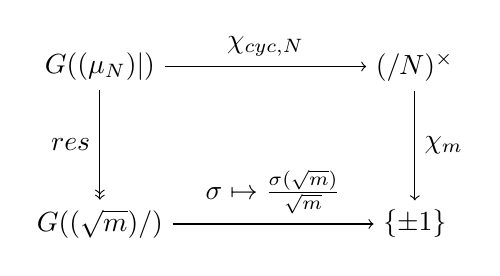
\begin{tikzpicture}[scale =1]
\node (D1) at (0,2)  {$G(\Q(\mu_N) | \Q)$};
\node (D3) at (4,2)  {$(\Z/N\Z)^\times$};
\node (D5) at (0,0)  {$G(\Q(\sqrt{m}) / \Q)$};
\node (D7) at (4,0)  {$\{\pm 1\}$};

\draw[->] (D1) -> (D3) node[midway, above]{$\isom{\chi_{cyc,N}}$};
\draw[->] (D5) -> (D7) node[midway, above]{$\sigma \mapsto \frac{\sigma(\sqrt{m})}{\sqrt{m}}$};
\draw[->] (D3) -> (D7) node[midway, right]{$\chi_m$};
\draw[->>] (D1) -> (D5) node[midway, left]{$res$};
%\draw [ultra thick, right hook->,    blue] (0,-1) -- (3,-1);
\end{tikzpicture}
\end{center}

\Satz{}
Sei $m$ quadratfrei und $N = 
\left\lbrace\begin{aligned}
\bet{m} && m \equiv 1 \mod{4}\\
4\bet{m} && m \equiv 2,3 \mod{4}
\end{aligned}\right.$\\
$p$ sei eine zu $N$ teilerfremde Primzahl. Es gilt
\[ p \text{ ist voll zerlegt in } \Q(\sqrt{m}) \Gdw{} \chi_m(p) = 1 \]

\Satz{Gaußsches Quadratisches Reziprozitätsgesetz}
Für zwei ungerade, verschiedene Primzahlen $p,q$ gilt
\[ \Leg{q}{p} = (-1)^{\frac{q-1}{2} \cdot \frac{p-1}{2} } \Leg{p}{q} \]

\paragraph{Ergänzungssätze}
\[ \Leg{-1}{p} = (-1)^{\frac{p-1}{2}} \text{ und } \Leg{2}{p} = (-1)^{\frac{p^2-1}{8}} \]

\Def{}
Sei $K$ ein Zahlkörper. Ein Element $a \in K^\times$ heißt \df{total positiv}, falls für alle reellen Stellen $\iota : K \inj{} \R$ gilt
\[ \iota(a) > 0 \]

\Satz{Strahlklassenkörper}
Sei $K$ ein Zahlkörper und $0\neq \af \subset \O_K$ ein Ideal.
\begin{itemize}
\item Es existiert genau eine endliche Körpererweiterung $K(\af)|K$, die folgende Eigenschaften für jedes Ideal $\pf \subset \O_K$ erfüllt
\begin{itemize}
\item $\pf\nmid \af$ $\Impl{}$ $\pf$ ist unverzweigt in $K(\af)$.
\item $\pf$ zerlegt sich voll in $K(\af)$ $\Gdw{}$ es existiert ein total positives $\alpha \in 1 + \af$ mit $\pf = (\alpha)$.
\end{itemize}
Wir nennen in diesem Fall $K(\af)$ den \df{Strahlklassenkörper} $\mod{\af}$.
\item $K(\af) /K$ ist abelsch und jede endliche abelsche Erweiterung ist in einem Strahlklassenkörper enthalten.
\item $\bf \subset \af \Gdw{} K(\bf) \supset K(\af)$
\item Für jede endliche abelsche Erweiterung $L|K$ existiert ein Ideal $\ff \subset \O_K$, das maximal ist mit der Eigenschaft $L\subset K(\ff)$. Dieses Ideal nennen wir den \df{Führer} der Erweiterung $L|K$.\\
Für jedes Ideal $\pf \subset \O_K$ gilt:
\[ \pf \text{ verzweigt in } L \Gdw{} \pf | \ff \] 
\end{itemize}

\section{Abstrakte bzw. Axiomatische Klassenkörpertheorie}
\Def{Stetiger $G$-Modul}
Sei $K$ ein Körper und $G := G_K := G(\overline{K}|K)$ die Galoisgruppe der maximalen separablen Erweiterung von $K$.\\
Eine abelsche, multiplikativ geschriebene Gruppe $A$ heißt \df{stetiger $G$-Modul}, falls eine stetige Rechtswirkung von $G$
\begin{align*}
G \times A & \Pfeil{} A\\
(\sigma, a) & \longmapsto a^\sigma
\end{align*}
gegeben ist, wobei $A$ hierbei mit der diskreten Topologie und $G$ mit der proendlichen Topologie ausgestattet wird, sodass folgende Eigenschaften erfüllt werden:
\begin{itemize}
\item $a^1 = a$
\item $(ab)^\sigma = a^\sigma b^\sigma$
\item $(a^\sigma)^\tau = a^{\sigma\tau}$
\item $A = \bigcup_{L|K \text{ endl.}}A_L$ wobei
\[A_L := A^{G_L} = \set{a\in A}{a^\sigma = a \forall \sigma \in G_L = G(\overline{L}|L)}\]
\end{itemize} 

\Def{Normabbildung}
Sei eine endliche Körpererweiterung $L'|L$ galoissch über $K$ gegeben. Definiere folgende \df{Normabbildung}
\begin{align*}
N_{L'|L} : A_{L'} & \Pfeil{} A_L\\
a & \longmapsto \prod_{\sigma \in G_L/G_{L'}}a^\sigma
\end{align*}
Ist $L'|L$ galoissch, so ist $A_{L'}$ ein $G(L'|L)$-Modul und es gilt
\[ A_{L'}^{G(L'|L)}  = A_L \]

\Def{Kohomologie}
Sei eine endliche, galoissche Körpererweiterung $L'|L$ galoissch über $K$ gegeben. Definiere folgende \df{Tate-Kohomologiegruppen}
\begin{align*}
H^0(G(L'|L), A_{L'} ) &:= A_L / N_{L'|L} A_{L'}\\
H\i (G(L'|L) , A_{L'}) &:= {}_{N_{L'|L}}A_{L'} / I_{G(L'|L)}A_{L'}
\end{align*}
wobei
\begin{align*}
{}_{N_{L'|L}}A_{L'} &:= \{a \in A_{L'}~|~N_{L'|L}(a) = 1\}\\
I_{G(L'|L)}A_{L'} &:= \{a^{\sigma - 1}~|~a \in A_{L'}, \sigma \in G(L'|L)\}
\end{align*}
${}_{N_{L'|L}}A_{L'}$ nennen wir auch die \df{Normrestgruppe}.

\Def{Verlagerung}
Sei $G$ eine Gruppe und $H$ eine Untergruppe mit endlichen Index. $R = G/H$ bezeichne ein Repräsentantensystem der Linksnebenklassen von $H$, welches die 1 enthält.\\ Definiere die \df{Verlagerung} durch
\begin{align*}
Ver : G^{ab}& \Pfeil{} H^{ab}\\
[g] & \longmapsto \left[ \prod_{r \in R}g_r \right]
\end{align*}
wobei die $g_r$ hinreichend wohldefiniert sind durch
\[ gr = r'g_r \]
für ein $r' \in R$.

\Def{Normrestsymbol}
Sei eine endliche, galoissche Körpererweiterung $L|K$ gegeben. Definiere das \df{Normrestsymbol} durch
\[ (\_, L|K) : A_K \surj{} A_K/N{L|K}A_L \pfeil{\isom{}} G(L|K)^{ab} \]
Das Normrestsymbol erfüllt folgende Eigenschaften:
\begin{itemize}
\item[(A1)] Für alle $\sigma \in G_K$ kommutiert
\begin{center}
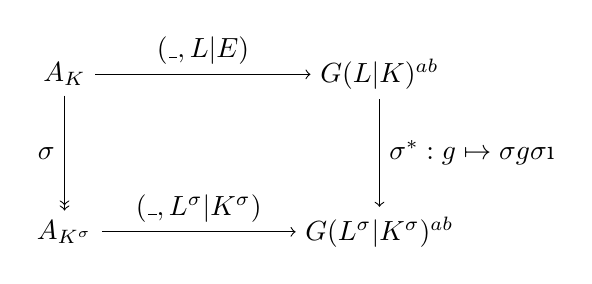
\begin{tikzpicture}[scale =1]
\node (D1) at (0,2)  {$A_K$};
\node (D3) at (4,2)  {$G(L|K)^{ab}$};
\node (D5) at (0,0)  {$A_{K^\sigma}$};
\node (D7) at (4,0)  {$G(L^\sigma|K^\sigma)^{ab}$};

\draw[->] (D1) -> (D3) node[midway, above]{$(\_, L|E)$};
\draw[->] (D5) -> (D7) node[midway, above]{$(\_, L^\sigma | K^\sigma)$};
\draw[->] (D3) -> (D7) node[midway, right]{$\sigma^* : g \mapsto \sigma g \sigma\i$};
\draw[->>] (D1) -> (D5) node[midway, left]{$\sigma$};
\end{tikzpicture}
\end{center}

\item[(A2)] Sei $K'|K$ eine endliche Erweiterung und setze $L' = K'L$. Dann kommutiert
\begin{center}
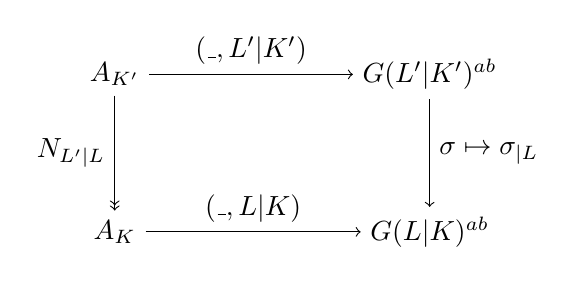
\begin{tikzpicture}[scale =1]
\node (D1) at (0,2)  {$A_{K'}$};
\node (D3) at (4,2)  {$G(L'|K')^{ab}$};
\node (D5) at (0,0)  {$A_{K}$};
\node (D7) at (4,0)  {$G(L|K)^{ab}$};

\draw[->] (D1) -> (D3) node[midway, above]{$(\_, L'|K')$};
\draw[->] (D5) -> (D7) node[midway, above]{$(\_, L | K)$};
\draw[->] (D3) -> (D7) node[midway, right]{$\sigma \mapsto \sigma_{|L}$};
\draw[->>] (D1) -> (D5) node[midway, left]{$N_{L'|L}$};
\end{tikzpicture}
\end{center}

\item[(A3)] Liegen endliche Körpererweiterungen $L|K'|K$ vor, sodass $L$ und $K'$ galoissch über $K$ sind, so kommutiert
\begin{center}
\begin{tikzpicture}[scale =1]
\node (D1) at (0,2)  {$A_{K'}$};
\node (D3) at (4,2)  {$G(L|K')^{ab}$};
\node (D5) at (0,0)  {$A_{K}$};
\node (D7) at (4,0)  {$G(L|K)^{ab}$};

\draw[->] (D1) -> (D3) node[midway, above]{$(\_, L|K')$};
\draw[->] (D5) -> (D7) node[midway, above]{$(\_, L | K)$};
\draw[->] (D7) -> (D3) node[midway, right]{$Ver$};
\draw[right hook->] (D5) -> (D1) node[midway, left]{};
\end{tikzpicture}
\end{center}
\end{itemize}

\section{Haupttheoreme der Klassenkörpertheorie}
\Def{Lokaler Körper}
Unter einem \df{lokalen Körper} verstehen wir $\R$ oder $\C$ oder einen vollständigen, diskret bewerteten Körper mit endlichem Restklassenkörper.

\Satz{Lokale Klassenkörpertheorie}
Sei $K$ ein lokaler Körper.
\begin{itemize}
\item Es existiert genau ein stetiger Gruppenhomomorphismus
\[ \phi_K : K^\times \Pfeil{} G_K^{ab} \]
der folgende Eigenschaften erfüllt:
\begin{itemize}
\item Für jede endliche, abelsche Erweiterung $L|K$ induziert $\phi_K$ einen Isomorphismus
\[ K^\times / N_{L|K} L^\times \Pfeil{\isom{}} G(L|K) \]
\item Ist $K\neq \R,\C$ und besitzt den endlichen Restklassenkörper $\kappa$, so kommutiert folgendes Diagramm
\begin{center}
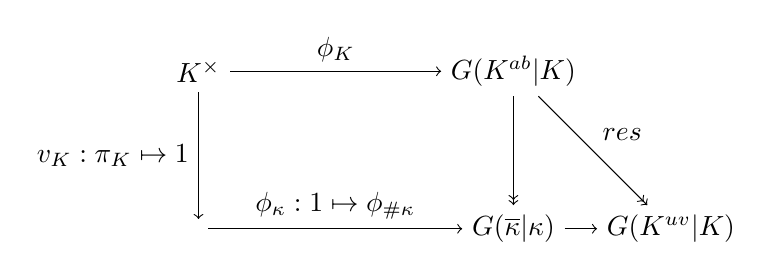
\begin{tikzpicture}[scale =1]
\node (D1) at (0,2)  {$K^\times$};
\node (D3) at (4,2)  {$G(K^{ab}|K)$};
\node (D5) at (0,0)  {$\Z$};
\node (D7) at (4,0)  {$G(\overline{\kappa}|\kappa)$};
\node (D9) at (6,0)  {$G(K^{uv}|K)$};

\draw[->] (D1) -> (D3) node[midway, above]{$\phi_K$};
\draw[->] (D5) -> (D7) node[midway, above]{$\phi_\kappa : 1 \mapsto \phi_{\#\kappa}$};
\draw[->>] (D3) -> (D7) node[midway, right]{};
\draw[->>] (D3) -> (D9) node[midway, above right]{$res$};
\draw[->] (D7) -> (D9) node[midway, above]{$\isom{}$};
\draw[->] (D1) -> (D5) node[midway, left]{$v_K:\pi_K\mapsto 1$};
\end{tikzpicture}
\end{center}
wobei $K^{ab}$ die maximale abelsche Erweiterung von $K$ und $K^{uv}$ ihre maximale unverzweigte Teilerweiterung ist.
\end{itemize}
\item Es ergeben sich folgende Korrespondenzen
\begin{center}
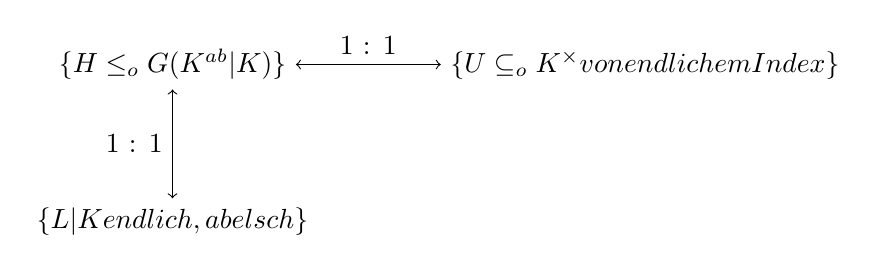
\begin{tikzpicture}[scale =2]
\node (D1) at (0,1)  {$\{H\leq_o G(K^{ab}|K)\}$};
\node (D3) at (3,1)  {$\{ U \subseteq_o K^\times \text{ von endlichem Index} \}$};
\node (D7) at (0,0)  {$\{ L |K \text{ endlich, abelsch} \}$};

\draw[<->] (D1) -> (D3) node[midway, above]{1 : 1};
\draw[<->] (D7) -> (D1) node[midway, left]{1 : 1};
%\draw [ultra thick, right hook->,    blue] (0,-1) -- (3,-1);
\end{tikzpicture}
\end{center}
\end{itemize}

\Def{Globale Körper}
Unter einem \df{globalen Körper} verstehen wir einen Zahl- bzw. Funktionenkörper.

\Satz{Globale Klassenkörpertheorie}
Sei $K$ ein globaler Körper, $C_K$ bezeichne seien Idelegruppe.
\begin{itemize}
\item Es existiert genau ein stetiger Gruppenhomomorphismus
\[ \phi_K : C_K \Pfeil{} G_K^{ab} \]
sodass für jede Stelle $v$ von $K$ folgendes Diagramm kommutiert
\begin{center}
\begin{tikzpicture}[scale =1]
\node (D1) at (0,2)  {$K_v^\times$};
\node (D3) at (4,2)  {$G(K_v^{ab}|K_v)$};
\node (D5) at (0,0)  {$C_K$};
\node (D7) at (4,0)  {$G(K^{ab}|K)$};

\draw[->] (D1) -> (D3) node[midway, above]{$\phi_{K_v}$};
\draw[->] (D5) -> (D7) node[midway, above]{$\phi_K : ? \mapsto \Frob_v$};
\draw[right hook->] (D3) -> (D7) node[midway, right]{};
\draw[right hook->] (D1) -> (D5) node[midway, left]{$\pi_v \mapsto ?$};
\end{tikzpicture}
\end{center}
wobei $K_v$ die Komplettierung von $K$ bzgl. $v$ bezeichnet. 

\item Für jede endliche, abelsche Erweiterung $L|K$ induziert $\phi_K$ einen Isomorphismus
\[ C_K / N_{L|K} C_L \Pfeil{\isom{}} G(L|K) \]

\item Es ergeben sich folgende Korrespondenzen
\begin{center}
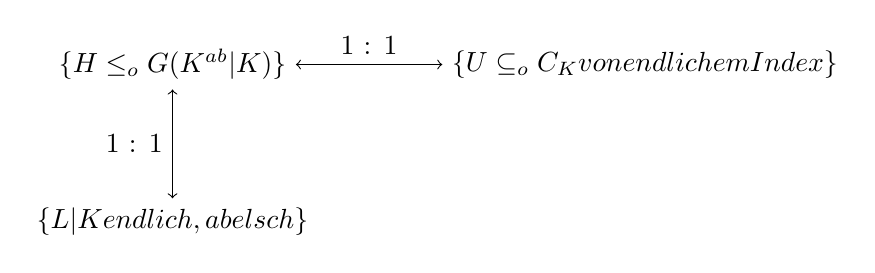
\begin{tikzpicture}[scale =2]
\node (D1) at (0,1)  {$\{H\leq_o G(K^{ab}|K)\}$};
\node (D3) at (3,1)  {$\{ U \subseteq_o C_K \text{ von endlichem Index} \}$};
\node (D7) at (0,0)  {$\{ L |K \text{ endlich, abelsch} \}$};

\draw[<->] (D1) -> (D3) node[midway, above]{1 : 1};
\draw[<->] (D7) -> (D1) node[midway, left]{1 : 1};
%\draw [ultra thick, right hook->,    blue] (0,-1) -- (3,-1);
\end{tikzpicture}
\end{center}
\end{itemize}

\section{Was besagt die Klassenkörpertheorie? Erste Folgerungen der Hauptresultate}
\Satz{}
Sei $L|K$ eine endliche, abelsche Erweiterung globaler Körper. $v$ sei eine Stelle von $K$, $\pi_v \in \O_{K_v} \subset K_v$ die zugehörige lokale Stelle. Definiere folgende Abbildung
\[ \Theta : K_v^\times \Inj{} C_K \Pfeil{} C_K/N_{L|K}C_L \]
Dann gilt
\begin{itemize}
\item $v$ zerlegt sich voll in $L$ $\Gdw{}$ $\Theta(K_v^\times) = \{1\}$
\item Ist $v$ endlich, so gilt
\[ v \text{ ist unverzweigt in }L\Gdw{} \Theta(\O_{K_v}^\times) = \{1\} \]
\item Sei $v$ endlich und unverzweigt in $L$. Dann liegt folgende Isomorphie vor
\begin{align*}
C_K / N_{L|K}C_L &\Pfeil{} G(L|K)\\
\Theta(\pi_v) & \longmapsto \Frob_v
\end{align*}
\end{itemize}